\documentclass[10pt]{beamer}

\usetheme{Frankfurt}

%%% Работа с русским языком
\usepackage{cmap}					% поиск в PDF
\usepackage{mathtext} 				% русские буквы в формулах
\usepackage[T2A]{fontenc}			% кодировка
\usepackage[utf8]{inputenc}			% кодировка исходного текста
\usepackage[english,russian]{babel}	% локализация и переносы
\usepackage{indentfirst}
\frenchspacing


%%% Дополнительная работа с математикой
\usepackage{amsmath,amsfonts,amssymb,amsthm,mathtools} % AMS
\usepackage{icomma} % "Умная" запятая: $0,2$ --- число, $0, 2$ --- перечисление

%% Номера формул
%\mathtoolsset{showonlyrefs=true} % Показывать номера только у тех формул, на которые есть \eqref{} в тексте.
%\usepackage{leqno} % Нумерация формул слева

%% Свои команды
\DeclareMathOperator{\sgn}{\mathop{sgn}}

%% Перенос знаков в формулах (по Львовскому)
\newcommand*{\hm}[1]{#1\nobreak\discretionary{}
	{\hbox{$\mathsurround=0pt #1$}}{}}

%%% Работа с картинками
\usepackage{graphicx}  % Для вставки рисунков
\graphicspath{{images/}}  % папки с картинками
\setlength\fboxsep{3pt} % Отступ рамки \fbox{} от рисунка
\setlength\fboxrule{1pt} % Толщина линий рамки \fbox{}
\usepackage{wrapfig} % Обтекание рисунков текстом
\usepackage{subfigure}

%%% Работа с таблицами
\usepackage{array,tabularx,tabulary,booktabs} % Дополнительная работа с таблицами
\usepackage{longtable}  % Длинные таблицы
\usepackage{multirow} % Слияние строк в таблице

%%% Программирование
\usepackage{etoolbox} % логические операторы

%
%\usepackage{fancyhdr} % Колонтитулы
% 	\pagestyle{fancy}
%\renewcommand{\headrulewidth}{0pt}  % Толщина линейки, отчеркивающей верхний колонтитул
% 	\lfoot{Нижний левый}
% 	\rfoot{Нижний правый}
% 	\rhead{Верхний правый}
% 	\chead{Верхний в центре}
% 	\lhead{Верхний левый}
%	\cfoot{Нижний в центре} % По умолчанию здесь номер страницы

\usepackage{setspace} % Интерлиньяж
%\onehalfspacing % Интерлиньяж 1.5
%\doublespacing % Интерлиньяж 2
%\singlespacing % Интерлиньяж 1

\usepackage{lastpage} % Узнать, сколько всего страниц в документе.

\usepackage{soul} % Модификаторы начертания


\usepackage{csquotes} % Еще инструменты для ссылок

%\usepackage[style=authoryear,maxcitenames=2,backend=biber,sorting=nty]{biblatex}

\usepackage{multicol} % Несколько колонок

\usepackage{tikz} % Работа с графикой
\usepackage{pgfplots}
\usepackage{pgfplotstable}

\renewcommand{\phi}{\varphi}
\renewcommand{\epsilon}{\varepsilon}
\usepackage[backend=biber, sorting=none]{biblatex}
\usepackage{subfigure}
\usepackage{authblk}

\addbibresource{lit.bib}

\theoremstyle{definition}
\newtheorem*{Def}{Definition}
\theoremstyle{plain}
\newtheorem{Lem}{Lemma}
\newtheorem{Th}{Theorem}

\newcommand{\delayV}[1]{\overset{\leftarrow}{\mathbf{x}}_{#1}}
\newcommand{\delayM}[1]{\overset{\leftarrow}{\mathbf{X}}_{#1}}

\title{Tensor decomposition and forecast for multidimensional time series}

\author[1]{Semkin Kirill}
\author[2]{Strijov Vadim}

\affil[1]{{\footnotesize Moscow Institute of Physics and Technology, semkin.ki@phystech.edu}}
\affil[2]{{\footnotesize Moscow Institute of Physics and Technology, strijov@ccas.ru}}

\date{}

\begin{document}
	
	\maketitle
	
	\begin{abstract}
		
		Processing of multidimensional time series is associated with additional task of modeling interconnections between signals. Its ignorance may cause incorrectness of any method's outcomes. On the other hand, taking this dependencies into account makes models larger and less interpretable as well as series analysis more narrow. A non-parametric method based on tensor data representation and SSA approach is proposed in the paper. Then, series decomposition technique and forecast type and formula were derived. Finally, elaborated theory was applied to electricity consumption and weather data. Obtained results were compared with mSSA, VAR, RNN models.
		
	\end{abstract}
	
	\textbf{Key words}: {\small time series, decomposition, forecast, SSA, CPD}.
	
	\section{Introduction}\label{Intro}
	
	The main object of the paper is multidimensional time series --- a set of observed signals $ \{x_i(t)\}_{i=1}^m $ where $ t \in 1 \ldots N $. %By series decomposition we mean additive expansion of each signals into several components.
	
	Decomposition~\cite{enders2010applied, x11, cleveland90} and forecast~\cite{3b1355aedd1041f1853e609a410576f3, enders2010applied, Box_Jenkins_methodology} methods for sole signal can not be directly transferred to set of signals if their behavior is interconnected. For instance, let's take predator-prey model~\cite{Volterra:1928}. The size of one population is dependent on another's and vice-versa. We are further assuming this connection to exist and will give formal definitions in the scope of particular models. 
	
	First, RNN model~\cite{neco, TEALAB2018334} links series with each other and their past values through composition of many nonlinear transformations. This information is encapsulated in hidden vector at each step. With that, one is able to forecast future values.
	
	Second, vector autoregression (VAR)~\cite{VAR_model1, doi:10.1080/01621459.1962.10480664} is a linear stochastic model for multidimensional signals. Denoting vector $ \mathbf{x}_t = (x_1(t) \ldots x_m(t))^{\mathsf{T}} $ as a series realizations at time $ t $, the further dynamics is following:
	
	\begin{equation*}
		\mathbf{x}_t = \boldsymbol{\mu} + \sum\limits_{i = 1}^p A_i \mathbf{x}_{t - i} + \mathbf{u}_t
	\end{equation*}
	
	Here  $ \boldsymbol{\mu} $ --- some constant vector, $ A_i $ are matrices $ m \times m $, $ \mathbf{u}_t $ is a random vector (e.g. white noise $ \text{WN}(t) $). Signal's connection is defined by $ A_i $ transformations, so again each series is dependent on each other and the whole past \textit{linearly}.
	
	Revised solutions allow to make predictions, but have quite a number of hyperparameters to be tuned. They also require exhaustive learning procedures. Furthermore, their structure does not contain explicit way of making series decomposition.
	
	To tackle listed issues, we developed a new method called tSSA which has only two adjustable variables. Computing tensor Canonical polyadic decomposition (CPD) is the only requirement for forecast and decomposition. Next, the approach is an extension of SSA method~\cite{ecfb9dc578be43ae9ee8fc88b8ff9151} for multidimensional time series. Due to that, its theory will be based on dynamical systems subtopic --- \textit{signal subspace}~\cite{1572261550523548160}. The main idea here is to build a phase representation of the observed signals (fig. \ref{pic:phase_traj}).
	
	In the end, we should mention another SSA modification --- mSSA~\cite{mSSA_overview}. In contrast, it operates with data only in a way of matrices and matrix decomposition. Nonetheless, both methods share same ideas in forecast and decomposition techniques.
	
	\begin{figure}[h]
		\centering
		\includegraphics[width=0.9\textwidth, keepaspectratio]{../../figs/phase_traj.png}
		\caption{Time series's phase trajectory visualization }\label{pic:phase_traj}
	\end{figure}
	
	The rest of the paper covers the theory and application of our method on the real data. Firstly, the mathematical model will be introduced and basis search in the signal space problem will be stated and resolved. These results will enable us to propose a way of decomposing the signals and make a forecast. Simultaneously, features of obtained solutions will be examined and result in two theorems. Finally, tSSA and mentioned methods will be applied on two datasets: electricity consumption and meteorology observations. We will obtain signal's predictions and additive decompositions. For the latter a special metric will be formulated. All results will be backed with figures and discussion.
	
	\section{Problem statement}\label{sec:problem_statement}
	
	Let us have observed multidimensional time series $ \{x_i(t)\}_{i=1}^m $ generated by some \emph{dynamical system} $ f $. By that we mean a law of coordinates $ \mathbf{y} \in X $ evolution in discrete time:
	
	\begin{gather*}
		\mathbf{y}(t + 1) = f(\mathbf{y}(t)), \ t \in \mathbb{N} \\
		\mathbf{y}(0) = \mathbf{y}_0
	\end{gather*}
	
	Here $ X $ is generally a high dimensional smooth manifold. Then, each trajectory of the system spawns our signals through unknown mapping $ \boldsymbol{\phi}: X \to \mathbb{R}^m $:
	
	\begin{equation*}
		\boldsymbol{\phi}(\mathbf{y}(t)) = \mathbf{x}_t \Leftrightarrow \begin{cases}
			\phi_1(\mathbf{y}(t)) = x_1(t) \\
			\ldots \\
			\phi_m(\mathbf{y}(t)) = x_m(t) \\
		\end{cases}
	\end{equation*}
	
	After that, it is hypothesized that trajectories $ \mathbf{y}(t) $ actually lie in a smaller dimension manifold $ M \subset X $. So now we should find an embedding of $ M $ into $ \mathbb{R}^{L} $ for some $ L $ and discover a basis in the image of the embedding. Having done that, we will obtain characterization of the initial system in terms of the standard linear space. The same will be equally applied to all $ x_i(t) $.
	
	\subsection*{One signal case}
	
	Our future approach roots from SSA method and Takens's theorem~\cite{citeulike:2735031}. Let's describe it in short. The theorem provides a solution for the stated problem in case of single series: any point $ \mathbf{y}(t) \in M $ we associate with the following vector:
	
	\[
	( \, \boldsymbol{\phi} \circ f^{t - L + 1}(\mathbf{y}(t)), \ldots , \boldsymbol{\phi} \circ f(\mathbf{y}(t)), \boldsymbol{\phi} \circ \mathbf{y}(t) \,)^{\mathsf{T}} = (x(t - L + 1), \ldots , x(t-1), x(t))^{\mathsf{T}}
	\] 
	
	It is called \emph{delay vector} in time $ t $ and denoted as $ \delayV{t} $. Their dimensionality $ L $ should satisfy $ L > 2 \cdot \dim(M) $. Function $ \phi(\cdot) $ should also meet some regularity conditions which are assumed to be fulfilled.
	
	So, with signal $ x(t) $ of length $ N $ we build $ N - L + 1 $ delay vectors. Corresponding embedding space $ \text{Lin}(\{\delayV{t}\}) $, so called \emph{signal subspace}, must be low dimensional, meaning $ \text{Lin}(\{\delayV{t}\}) \subset \mathbb{R}^L $. Orthonormed basis here is a SVD's $ U $-component of \emph{trajectory matrix} $ \mathbf{H}_x $ which is build from delay vectors:
	
	\[
		\mathbf{H}_x = [ \delayV{1} \ldots  \delayV{N - L + 1}]
	\]
	
	\subsection*{Series interconnection and tSSA method}\label{sec:tssa_method}
	
	Теперь обобщим данный подход на несколько временных рядов.
	
	Now let's generalize previous results for the multiple series.
	
	\begin{figure}[h]
		\centering
		\subfigure{\includegraphics[width=0.4\textwidth, keepaspectratio]{../../figs/Trajectory_Tensor_1}}
		\subfigure{\includegraphics[width=0.4\textwidth, keepaspectratio]{../../figs/Trajectory_Tensor_2}}
		
		\caption{Two views on trajectory tensor. The left is in terms of signals' trajectory matrices $ \{x_i(t)\}_{i=1}^m $. The right is in terms of delay matrices.}\label{pic:traj_tensor}
	\end{figure}
	
	In this case $ \boldsymbol{\phi}(\cdot) $ is multidimensional. So instead of the single delay vector we should consider their set for all $ m $ signals in time $ t $. That means the embedding image now contains so called \emph{delay matrices} $ ( \delayV{1_t} \ldots \delayV{m_t} ) := \delayM{t} $. Next, instead of trajectory matrix we should introduce \textit{trajectory tensor} $ \mathbf{T} $. It is constructed  by putting delay matrices along the second dimension of the tensor, fig. \ref{pic:traj_tensor} (left). This procedure is equivalent to the one for $ \mathbf{H}_x $. But our tensor has an important property: $ \mathbf{T} $ can also be built as an alignment of signals' trajectory matrices $ \mathbf{H}_{x_i} $ along the third dimension, fig. \ref{pic:traj_tensor} (right).
	
	Then, reasoning analogues to the one signal case we obtain \emph{signals' set subspace} as a linear span of delay matrices. But we were supposed to built the subspace for each signal individually.
	
	It's time to give a definition for signals' interrelation in our model's scope.
	
	\begin{Def}		
		We call a set of time series \emph{interconnected} if they all share the common subspace with the same basis.
	\end{Def}
	
	Now we are ready to find this shared elements for signals. Note that to do so we just need to decompose each signal's trajectory matrix through the same set of factors. Finally, let's apply CPD to our trajectory tensor and have a look at its slices by third dimension.
	
	\begin{equation}\label{eq:tSSA_decomp}
		\mathbf{T} = \sum\limits_{i = 1}^{r} \mathbf{a}_i \otimes \mathbf{b}_i \otimes \mathbf{c}_i \Leftrightarrow \begin{cases}
			\mathbf{H}_{x_1} = \sum\limits^{r} \boldsymbol{\sigma}_{x_1}(i) \cdot \mathbf{a}_i  \mathbf{b}_i^{\mathsf{T}}  \\
			\mathbf{H}_{x_2} = \sum\limits^{r} \boldsymbol{\sigma}_{x_2}(i) \cdot \mathbf{a}_i  \mathbf{b}_i^{\mathsf{T}} \\
			\ldots \\
			\mathbf{H}_{x_m} = \sum\limits^{r} \boldsymbol{\sigma}_{x_m}(i) \cdot \mathbf{a}_i  \mathbf{b}_i^{\mathsf{T}} 
		\end{cases}
	\end{equation}
	
	What have we got? CPD is defined by tensor rank $ r $ and a set of vectors which we can pack in matrices: $ A = [\mathbf{a}_1 \ldots \mathbf{a}_r]; B = [\mathbf{b}_1 \ldots \mathbf{b}_r]; C = [\mathbf{c}_1 \ldots \mathbf{c}_r] $. Row $ k $ of matrix $ C $ is denoted as $ \boldsymbol{\sigma}_{x_k} $. It has the sense of singular values but can be negative.
	
	After, from CPD definition as a (\ref{eq:tSSA_decomp}) kind decomposition with minimal $ r $ we can derive that $ A, B, C $ are full-rank matrices. So, signals' shared subspace is  $ \text{Lin}(\{\mathbf{a}_i\}) $ with unified basis $ \{\mathbf{a}_i\}_{i = 1}^r $ which is not orthonormed in general. Then, back in the problem statement we assumed dimensionality of the embedding to be rather small. Therefore relation $ r \ll L $ should be true.
	
	Lastly, let's note that \emph{rows} of $ \mathbf{H}_{x_k} $ are also delay vectors but have another dimension of $ N - L + 1 $. So the shared subspace for them would be $ \text{Lin}(\{\mathbf{b}_i\}) $. This result proves our approach to be consistent with choice of $ \delayV{k_t} $. As a remark, mSSA lacks such feature.
	
	What to the signals' link, it is regulated by $ \boldsymbol{\sigma}_{x_k} $. For instance, if all the rows have zero elements in non-overlapping positions then our built subspace breaks down into a direct sum of individual signal's subspaces. It is total link absence case. The exact opposite situation is when $ \boldsymbol{\sigma}_{x_k} $ are non-zero for all series.
	
	\subsection*{Time series decomposition}\label{sec:decomposition}
	
	We can break series into several components using the conception: \emph{decomposition of trajectory matrix $ \mathbf{H}_{x_k} $ defines decomposition of related signal}. Its first part implies representation of $ \mathbf{H}_{x_k} $ as a sum of factors (\ref{eq:tSSA_decomp}). This technique comes from SSA. Because all matrices are similarly decomposed, we can focus on the task for a single series.
	
	Besides, we should point out the main feature of trajectory matrices --- \emph{hankelness}. That simply means equal elements along each anti-diagonal. Every series of length $ N $ bijectionly corresponds to hankel matrix of size $ L \times (N - L + 1) $.
	
	Now, decomposition procedure is following: we assume factors of $ \mathbf{H}_{x_k} $ to be able to pack in $ s $ groups in a special way. That means if we sum all factors within each group the result matrices $ C_1, \ldots, C_s $ will be hankel. This situation would perfectly correspond to representation of $ x_k(t) $ as a sum of $ s $ signals. Unfortunately, it is almost infeasible even with trivial series \cite{ecfb9dc578be43ae9ee8fc88b8ff9151}, so every $ C_i $ should be additionally \emph{hankelized}. This operation average each matrix's anti-diagonal so it becomes hankel. Let's denote the operator as $ \text{Hankel}(\cdot) $. 
	
	The whole algorithm can be written as a chain of identical expressions:
	
	\begin{multline}\label{eq:decomp_method_ideal}
		\underline{\mathbf{H}_{x_k}} \overset{1}{=} \sum\limits_{i = 1}^{r} \boldsymbol{\sigma}_{x_k}(i) \cdot \mathbf{a}_i  \mathbf{b}_i^{\mathsf{T}} \overset{2}{=} \sum\limits_{i \in \mathbb{I}_1} \boldsymbol{\sigma}_{x_k}(i) \cdot \mathbf{a}_i  \mathbf{b}_i^{\mathsf{T}} + \ldots + \sum\limits_{i \in \mathbb{I}_s} \boldsymbol{\sigma}_{x_k}(i) \cdot \mathbf{a}_i  \mathbf{b}_i^{\mathsf{T}} \overset{3}{=} \\ \overset{3}{=} C_1 + \ldots + C_s \overset{4}{=} \underline{\text{Hankel}(C_1) + \ldots + \text{Hankel}(C_s)}  \Leftrightarrow x_k(t) = c_1(t) + \ldots c_s(t)
	\end{multline}
	
	Here $ \mathbb{I}_1 \sqcup \ldots \sqcup \mathbb{I}_s = \{1, \ldots, r\} $ --- chosen groups of indices. Actually, the forth equality needs some extra validation. To make it, first consider hankel operator's property:
	
	\begin{Lem}
		$ \text{Hankel}(\cdot) $ operator is linear.
	\end{Lem}
	
	\begin{proof}		
		Having matrices $ A $ and $ B $ with the same size, let's look at their elements from one anti-diagonal $ a_1, \ldots, a_n $ and $ b_1, \ldots, b_n $. Then this anti-diagonal in $ \text{Hankel}(A + B) $ is written as $ \dfrac{1}{n} \sum\limits^n (a_i + b_i) = \dfrac{1}{n} \sum\limits^n a_i + \dfrac{1}{n} \sum\limits^n b_i $, resulting in a sum of  $ \text{Hankel}(A) $ and $ \text{Hankel}(B) $ anti-diagonals.
		
		Secondly, having a scalar $ \alpha $ it is also trivial that $ \dfrac{1}{n} \sum\limits^n \alpha \cdot a_i = \alpha \dfrac{1}{n} \sum\limits^n a_i $. Then we finally derive $ \text{Hankel}(\alpha A) = \alpha \text{Hankel}(A) $.
	\end{proof}
	
	Returning to forth equality in (\ref{eq:decomp_method_ideal}), we can combine this lemma and the fact that $ \mathbf{H}_{x_k} $ is itself hankel to get a complete justification. This outputs in the correctness of series decomposition procedure for any chosen grouping of factors.
	
	\subsection*{Optimal decomposition and its computational complexity}\label{sec:optimal_decomp}
	
	Несмотря на корректность имеющегося алгоритма, хочется группировать факторы так, что каждая матрица $ C_i $ была как можно более "<ганкелевой">. Это соответствует сформулированному принципу о связи разложения матриц и сигналов, а также повышает интерпретируемость компонент. Опишем задачу формально и исследуем её.
	
	Рассмотрим первое равенство в (\ref{eq:decomp_method_ideal}), а также применим к нему оператор ганкелизации:
	
	\begin{equation*}
		\begin{cases*}
			\mathbf{H}_{x_k} = \sum\limits_{i = 1}^{r} \boldsymbol{\sigma}_{x_k}(i) \cdot \mathbf{a}_i  \mathbf{b}_i^{\mathsf{T}} \\
			\mathbf{H}_{x_k} = \sum\limits_{i = 1}^{r} Hankel(\boldsymbol{\sigma}_{x_k}(i) \cdot \mathbf{a}_i  \mathbf{b}_i^{\mathsf{T}})
		\end{cases*}
	\end{equation*}
	
	Ещё раз напомним, что $ \mathbf{H}_{x_k} $ ганкелева по построению. Вычтем из первого втрое и обозначим $ H_i = \boldsymbol{\sigma}_{x_k}(i) \cdot \mathbf{a}_i  \mathbf{b}_i^{\mathsf{T}} - Hankel(\boldsymbol{\sigma}_{x_k}(i) \cdot \mathbf{a}_i  \mathbf{b}_i^{\mathsf{T}}) $, что соответствует невязке между исходной матрицей и её ганкелизацией. Т.о. получим:
	
	\begin{equation}\label{eq:residuals_equation}
		H_1 + \ldots + H_r = 0 \Leftrightarrow H_r = - \sum\limits_{j = 1}^{r - 1} H_j
	\end{equation}
	
	Теперь группировка факторов и ганкелевость итоговых матриц $ C_i $ (см. предыдущий подраздел) становится равносильна следующему: $ \sum_{k \in \mathbb{I}_i} H_k = 0, \  \forall i \in 1, \ldots, s $. Т.е. матрицы невязок суммируются в ноль внутри каждой группы. Далее, несложно заметить, что если существует разложение на $ s $ групп, то к нему можно прийти, разделяя имеющиеся группы факторов на две последовательно. Поэтому остановимся на этой упрощённой задаче.
	
	Из (\ref{eq:residuals_equation}) видно, что все матрицы невязок уже суммируются в $ 0 $, т.е. группу для $ H_r $ можно определить, сгруппировав оставшиеся невязки. Введём для каждой из них переменную-индикатор $ \beta_j \in \{0, 1\} $, показывающую, к какой из двух групп относится невязка. 
	
	Итак, ещё раз перечислим все условия. $ H_i $ в одной группе суммируются в $ 0 $; также считаем, что все они ненулевые (иначе мы уже имеем искомую группировку), т.е. в группе должно быть хотя бы две невязки. Т.о. задача поиска группировки свелась к следующей:
	
	\begin{equation}
		\begin{cases*}
			\sum\limits_{j = 1}^{r - 1} \beta_j H_j = 0 \\
			\beta_j \in \{0, 1\}, \ \forall j \in 1, \ldots, r \\
			\sum\limits_{i = 1}^{r - 1} \beta_j \ge 2
		\end{cases*}
	\end{equation}
	
	Для придания задаче более знакомого вида, во-первых, векторизуем каждую $ H_i $, и соберём все эти векторы в одну матрицу $ \Lambda $, а также введём $ \boldsymbol{\beta} = (\beta_1 \ldots \beta_{r-1}) $. Вспомним, что на практике мы не ждём идеальной ситуации суммирования в $ 0 $ матриц невязок (ганкелевости $ C_i $, см. предыдущий подраздел), нам достаточно сделать сумму как можно более близкой к нулю. Это приводит нас к конечной формулировке:
	
	\begin{equation}\label{eq:decomp_search_final}
		\begin{cases*}
			\lVert \Lambda \boldsymbol{\beta} \rVert \to \underset{\boldsymbol{\beta}}{\min} \\
			\beta_j \in \{0, 1\}, \ \forall j \in 1, \ldots, r \\
			\sum\limits_{i = 1}^{r - 1} \beta_j \ge 2
		\end{cases*}
	\end{equation}
	
	Назовём решение этой системы \emph{оптимальной декомпозицией ряда}. Она представляет из себя задачу наименьших квадратов с целочисленными ограничениями (ILS), которая, как показано в \cite{van1981another}, является NP-сложной. Все проведённые рассуждения приведём в виде:
	
	\begin{Th}
		Оптимальная декомпозиция ряда, в смысле поиска группировки факторов разложения траекторной матрицы ряда, является NP-сложной задачей.
	\end{Th}
	
	Несмотря на полученный результат, существуют методы и эвристики для сведения ILS к эффективно вычислим задачам, см. \cite{Grafarend2022}.
	
	
	\subsection*{Прогноз для набора рядов}\label{sec:tssa_forecast}
	
	Получение предсказания нашей модели сводится к восстановлению компонент векторов задержек каждого входного ряда. Т.к. мы построили общий для всех сигналов базис $ \{\mathbf{a}_i\}_{i = 1}^r $, то каждый сигнал может обрабатываться независимо.
	
	Если бы $ \{\mathbf{a}_i\}_{i = 1}^r $ был ортогональным, то мы бы могли применить технику прогнозирования SSA \cite{ecfb9dc578be43ae9ee8fc88b8ff9151}. Мы не имеем такой гарантии, поэтому процедуру необходимо модифицировать.
	
	Рассмотрим входной ряд $ x(t) $ и построим для него прогноз на один шаг вперёд. Вектор задержки $ \delayV{N + 1} = (x(N - L) \ldots x(N + 1))^{\mathsf{T}} $, в котором последняя компонента неизвестна, лежит в пространстве $ \text{Lin}(\{\mathbf{a}_i\}) $. В терминах вводимой ранее матрицы $ A \in \mathbb{R}^{L \times r} $ полного ранга (см. раздел \hyperref[sec:tssa_method]{Взаимосвязь рядов и метод tSSA}) это записывается как:
	
	\begin{align}\label{eq:main_pred_for_A}
		\delayV{N + 1} = A \boldsymbol{\lambda} &\Leftrightarrow \begin{cases}
			\mathbf{x}_{kn} = A_{kn} \boldsymbol{\lambda}  \\
			x(N + 1) = \mathbf{a}_{pr}^{\mathsf{T}} \boldsymbol{\lambda}
		\end{cases}, \text{ где } \\
		A &= \left( \dfrac{A_{kn}}{\mathbf{a}_{pr}^{\mathsf{T}}} \right) \nonumber \\
		\delayV{N + 1} &= (\mathbf{x}_{kn} \  x(N + 1))^{\mathsf{T}} \nonumber
	\end{align}
	
	Здесь $ \boldsymbol{\lambda} \in \mathbb{R}^r $; вектор задержки и матрица представлены в блочном виде, разделяющим известную часть сигнала (known) и его будущее значение (predicted). Для построения прогноза необходимо определить $ \boldsymbol{\lambda} $. 
	
	Матрица имеющейся СЛАУ $ A_{kn} \in \mathbb{R}^{(L - 1) \times r} $ имеет ранг не менее $ r - 1 $, но мы предположим, что удаление одной строчки оставит ранг полным. Как показывает практика, это необременительное условие. Сама система, в силу предположения модели $ r \ll L $, является переопределённой. Значит её решение разумно искать только в смысле наименьших квадратов: $ \boldsymbol{\lambda} = (A_{kn}^T A_{kn})^{-1} A_{kn}^T \mathbf{x}_{kn} $. В итоге прогноз модели даётся:
	
	\begin{equation}\label{eq:tssa_pred}
		x(N + 1) = \mathbf{a}_{pr}^{\mathsf{T}} (A_{kn}^T A_{kn})^{-1} A_{kn}^T \mathbf{x}_{kn}
	\end{equation}
	
	Здесь $ \mathbf{a}_{pr}^{\mathsf{T}} (A_{kn}^T A_{kn})^{-1} A_{kn}^T = \mathbf{d}^{\mathsf{T}} $ --- вектор-строка, и, вычислив её единожды, можно последовательно строить предсказания на произвольный горизонт вперёд.
	
	Теперь перепишем (\ref{eq:tssa_pred}) в терминах $ x(t) $:
	
	\begin{equation*}\label{eq:autoregr}
		x(t) = \sum\limits_{i = 1}^{L - 1} d_i \cdot x(t - i)
	\end{equation*}
	
	Это выражение приводит нас к окончательному выводу о характере прогноза:
	
	\begin{Th}
		Модель прогнозируемого методом tSSA ряда --- \textit{авторегрессионная} $ AR(L - 1) $. Поведение прогноза полностью определяется коэффициентами авторегрессии $ d_i $, найденными в (\ref{eq:tssa_pred}).
	\end{Th}
	
	\section{Вычислительный эксперимент}	
	
	\subsection*{Цели и постановка}
	
	В данном разделе мы рассмотрим применение метода tSSA для декомпозиции и прогноза нескольких многомерных временных рядов, а также сравним его с другими моделями, упомянутыми во введении: mSSA, VAR, RNN. Упомянем, что mSSA по теории и применению во многом схожа с нашим методом, с её помощью можно решать обе упомянутые задачи. Две другие модели способны только к предсказанию.
	
	Для измерения \textbf{качества декомпозиции} введём метрики:
	
	\begin{Def}
		\emph{Абсолютной ошибкой ганкелизации} матрицы M назовём 
		
		\[
		\text{AHE} = \lVert M - \text{Hankel}(M) \rVert_2
		\] 
		
	\end{Def}	
	
	\begin{Def}		
		
		\emph{Относительной ошибкой ганкелизации} матрицы M назовём 
		
		\[
		\text{RHE} = \frac{\text{AHE}}{\lVert M \rVert_2} 
		\] 		
		
	\end{Def}
	
	AHE можно представлять как суммарное стандартное отклонение антидиагоналей матрицы. RHE её более интерпретируемая модификация, которая и будет использоваться далее. 
	
	Напомним, что разложение ряда на компоненты эквивалентно группировке факторов разложения траекторной матрицы сигнала, т.е. получению матриц $ C_i $ (см. раздел \hyperref[sec:decomposition]{Декомпозиция набора рядов}). Именно для них мы и будем рассчитывать RHE, а также среднее RHE по одному ряду --- $ \overline{\text{RHE}}_{ts} $, и среднее RHE всех рядов датасета --- $ \overline{\text{RHE}} $.
	
	Для измерения \textbf{качества прогноза} ряда будем использовать стандартные метрики: среднеквадратическую ошибку $ \text{MSE}_{ts} $ и среднюю абсолютную процентную ошибку $ \text{MAPE}_{ts} $, а также их усреднения по всему датасету c обозначениями $ \overline{\text{MSE}} $ и $ \overline{\text{MAPE}} $.
	
	В качестве сигналов будут рассмотрены два набора данных: потребление электроэнергии и её цена за единицу мощности (рис. \ref{fig:electr_data}); а также три ряда, характеризующие погоду г. Берлин в период с 1980 по 1990 год: средние за день температура, осадки и атмосферное давление (рис. \ref{fig:weather_data}). Мы предполагаем наличие связи рядов в каждом наборе (на основе экономических/физических причин), т.к. это важное условие применения нашего метода (см. \hyperref[sec:tssa_method]{Взаимосвязь рядов и метод tSSA}). Каждый ряд имеет длину $ \approx 3 \cdot 10^3 $, из которых $ 20\% $ --- отложенная выборка для оценки качества прогноза.
	
	\begin{figure}[h]
		\centering
		\includegraphics[width=0.48\textwidth, keepaspectratio]{../../figs/Electricity_Production}
		\includegraphics[width=0.48\textwidth, keepaspectratio]{../../figs/Electricity_Price}
		\caption{Многомерный ряд потребления электричества и его цены за единицу мощности}\label{fig:electr_data}
	\end{figure}
	
	\begin{figure}[h]
		\centering
		\includegraphics[width=0.48\textwidth, keepaspectratio]{../../figs/Temperature.png}
		\includegraphics[width=0.48\textwidth, keepaspectratio]{../../figs/Precipitation.png}
		\includegraphics[width=0.48\textwidth, keepaspectratio]{../../figs/Pressure.png}
		\caption{Многомерный ряд физических величин: температуры, осадков и давления, измеренных на метеостанции г. Берлин}\label{fig:weather_data}
	\end{figure}
	
	Опишем нюансы применения метода tSSA. Во-первых, вычисление канонического ранга тензора --- NP-трудная задача \cite{HASTAD1990644}, поэтому каждый раз ранг разложения будет указываться явно. Во-вторых, используемый алгоритм CP-разложения --- ALS \cite{kolda_tensors}, имеет ошибку аппроксимации, из-за чего возникает неточность разложения траекторных матриц. Относительные величины этих невязок будут указаны ниже. В-третьих, для поиска декомпозиции рядов будет решаться задача ILS (\ref{eq:decomp_search_final}), в которой матрица имеет высокую строковую размерность. Для ускорения мы сократим её до нескольких сотен, что всё ещё будет много больше размерности искомого вектора параметров. Используемый солвер --- SCIP \cite{BolusaniEtal2024ZR}.
	
	Наконец, мы зафиксируем единый для всех моделей параметр, отвечающий за длину предуславливания методов на историю рядов, который обозначался за $ L $. Для tSSA и mSSA он был описан в начале раздела \ref{sec:problem_statement}; в RNN это можно считать длиной энкодера; в VAR это максимальная длина истории ряда, на которую производится авторегрессия. Везде ниже $ L = 500 $.		
	
	\subsection*{Результаты и обсуждение}
	
	Начнём с задачи прогнозирования. На рис. \ref{fig:mse_mape_electr} и \ref{fig:mse_mape_weather} отображена зависимость метрик качества прогноза tSSA в зависимости от ранга CP-разложения. Точка минимума и характер изменения MSE и MAPE совпадают. Наблюдается эффект переобучения при повышении значения ранга, особенно резкое ухудшение метрик у данных погоды. При этом ошибка CP-разложения монотонно убывает, см. рис. \ref{fig:cpd_errors}.
	
	\begin{figure}[h]
		\centering
		\includegraphics[width=0.48\textwidth, keepaspectratio]{../../experiments/electricity/tssa/figs/prediction/MSE_rank.png}
		\includegraphics[width=0.48\textwidth, keepaspectratio]{../../experiments/electricity/tssa/figs/prediction/MAPE_rank.png}
		\caption{Данные электроэнергии. Значения метрик $ \overline{\text{MSE}} $ и $ \overline{\text{MAPE}} $ предсказания tSSA для разных рангов CP-разложения. Отдельно выделен оптимальный ранг.}\label{fig:mse_mape_electr}
	\end{figure}
	
	\begin{figure}[h]
		\centering
		\includegraphics[width=0.48\textwidth, keepaspectratio]{../../experiments/weather/tssa/figs/prediction/MSE_rank.png}
		\includegraphics[width=0.48\textwidth, keepaspectratio]{../../experiments/weather/tssa/figs/prediction/MAPE_rank.png}
		\caption{Данные погодных условий. Значения метрик $ \overline{\text{MSE}} $ и $ \overline{\text{MAPE}} $ предсказания tSSA для разных рангов CP-разложения. Отдельно выделен оптимальный ранг.}\label{fig:mse_mape_weather}
	\end{figure}
	
	\begin{figure}[h]
		\centering
		\includegraphics[width=0.48\textwidth, keepaspectratio]{../../experiments/electricity/tssa/figs/CPD_error.png}
		\includegraphics[width=0.48\textwidth, keepaspectratio]{../../experiments/weather/tssa/figs/CPD_error.png}
		\caption{Относительные ошибки CPD-аппроксимации траекторных тензоров в зависимости от ранга разложения. Слева --- электроэнергии, справа --- погоды.}\label{fig:cpd_errors}
	\end{figure}
	
	Графики наилучшего прогноза tSSA приведены на рис. \ref{fig:tssa_electr_pred} и \ref{fig:tssa_weather_pred}, где наглядно видны различия метода с малым и большим рангом. В первом случае авторегрессионная модель прогноза большего порядка (см. теорему раздела \hyperref[sec:tssa_forecast]{Прогноз для набора рядов}), что позволяет точно аппроксимировать ряд. В случае же погоды большой порядок приводил к нестабильности и неограниченному росту, но при уменьшении степеней свободы возможно аппроксимировать сигналы только в среднем.
	
	Итоговые метрики качества прогноза всех моделей --- в табл. \ref{tab:pred_res_electr} и \ref{tab:pred_res_weather}. Наш метод показал наилучшие результаты, хотя mSSA был близок по точности. Метод VAR оказался нестабилен на выбранном горизонте прогнозирования, а RNN обучался в константную функцию.
	
	\def\arraystretch{1.1}
	\begin{table}[h]
		\centering
		\caption{Метрики моделей на прогнозировании данных электроэнергии}\label{tab:pred_res_electr}
		\begin{tabular}{|c|c|c|c|c|}
			\hline
			& \textit{tSSA}  & \textit{mSSA} & \textit{VAR} & \textit{RNN} \\ \hline
			$ \overline{\text{MSE}}_{\text{Producution}} $, $10^6$ & 1.24           & 1.51          & 7.81         & 2.70         \\ \hline
			$ \overline{\text{MSE}}_{\text{Price}} $, $10^3$      & 0.88           & 1.03          & 4.85         & 30.0         \\ \hline
			$ \overline{\text{MSE}} $, $10^6$             & \textbf{0.62}  & 0.75          & 3.91         & 135.00       \\ \hline
			$ \overline{\text{MAPE}}_{\text{Producution}} $        & 0.054          & 0.060         & 0.137        & 0.999        \\ \hline
			$ \overline{\text{MAPE}}_{\text{Price}} $             & 0.164          & 0.170         & 0.360        & 1.004        \\ \hline
			$ \overline{\text{MAPE}} $                    & \textbf{0.109} & 0.115         & 0.249        & 1.002        \\ \hline
		\end{tabular}
	\end{table}
	
	\def\arraystretch{1.1}
	\begin{table}[h]
		\centering
		\caption{Метрики моделей на прогнозировании данных погоды}\label{tab:pred_res_weather}
		\begin{tabular}{|c|c|c|c|c|}
			\hline
			& \textit{tSSA}                & \textit{mSSA} & \textit{VAR} & \textit{RNN} \\ \hline
			$ \overline{\text{MSE}}_{\text{Temp}} $  & 14.16                        & 20.12         & 40.67        & -            \\ \hline
			$ \overline{\text{MSE}}_{\text{Prec}} $  & 11.02                        & 11.23         & 22.84        & -            \\ \hline
			$ \overline{\text{MSE}}_{\text{Pres}} $  & 98.02                        & 101.23        & 156.75       & -            \\ \hline
			$ \overline{\text{MSE}} $        & \textbf{41.067}              & 44.193        & 73.420       & -            \\ \hline
			$ \overline{\text{MAPE}}_{\text{Temp}} $ & 0.850 & 0.626         & 0.468        & -            \\ \hline
			$ \overline{\text{MAPE}}_{\text{Prec}} $ & 3.151 & 2.834         & 4.637        & -            \\ \hline
			$ \overline{\text{MAPE}}_{\text{Pres}} $ & 0.007 & 1.254         & 3.983        & -            \\ \hline
			$ \overline{\text{MAPE}} $       & \textbf{1.336}               & 1.571         & 3.029        & -            \\ \hline
		\end{tabular}
	\end{table}
	
	Теперь рассмотрим задачу декомпозиции. На рис. \ref{fig:decomp_rhe_rank} представлены зависимости качества разложения от значения CP-ранга. В обоих случаях $ \overline{\text{RHE}} $ достаточно быстро достигает минимума, после чего не меняется или растёт. Вспоминая аналогичный результат для прогнозирования, можно сделать вывод, что метод tSSA достигает наибольшей обобщающей способности на небольших канонических рангах траекторных тензоров данных. В свою очередь, этот ранг пропорционален размерности собственного пространства сигналов (см. начало раздела \ref{sec:problem_statement}). Из этого заключаем о выполнении главной теоретической предпосылки для применения нашего метода.
	
	На рис. \ref{fig:electr_decomp_tssa} и \ref{fig:weather_decomp_tssa} представлены результаты наилучшей найденной декомпозиции рядов на две компоненты методом tSSA. В силу вычислительной сложности задачи ILS, разложение на б$\acute{\text{о}}$льшее количество компонент не производится. Из графиков видно, как сильно общий базис сигналов влияет на их декомпозицию: для генерации электроэнергии и её цены компоненты получились почти идентичными, с точностью до смещения и масштаба. Аналогичная ситуация для температуры и осадков в данных погоды, а для атмосферного давления разложение получилось другим. Далее, на рис. \ref{fig:weather_decomp_tssa} метод выделил для каждого сигнала по две периодические составляющие: одна из них большой амплитуды, другая много меньшей. Небольшой шум остался в каждой компоненте. На рис. \ref{fig:electr_decomp_tssa} метод выделил по два высокочастотных колебания разной амплитуды и смещения.
	
	Для сравнения на рис. \ref{fig:electr_decomp_mssa} и \ref{fig:weather_decomp_mssa} приведены результаты декомпозиции методом mSSA на пять компонент. Для их получения не было необходимости в решении ILS или настраивания CP-ранка, но они подбиралась вручную на основе близости сингулярных чисел некоторой матрицы, см. \cite{ecfb9dc578be43ae9ee8fc88b8ff9151}. Тем не менее компоненты получились более интерпретируемыми и подробными: метод выделил несколько трендов и гармоник. Также, как видно из табл. \ref{tab:decomp_electr_results} и \ref{tab:decomp_weather_results}, mSSA немного выиграл по точности. Т.о. вычислительная сложность декомпозиции tSSA является главной проблемой метода и требует разработки собственных эвристик, которые, к слову, у mSSA уже имеются \cite{ecfb9dc578be43ae9ee8fc88b8ff9151}.	
	
	\def\arraystretch{1.2}
	\begin{table}[h!]
		\centering
		\caption{Метрики моделей на декомпозиции данных электроэнергии}\label{tab:decomp_electr_results}
		\begin{tabular}{|c|c|c|}
			\hline
			& tSSA  & mSSA           \\ \hline
			$ \overline{\text{RHE}}_{\text{Producution}} $  & 0.507 & 0.308          \\ \hline
			$ \overline{\text{RHE}}_{\text{Price}} $      & 0.511 & 0.31           \\ \hline
			$ \overline{\text{RHE}} $             & 0.509 & \textbf{0.309} \\ \hline
		\end{tabular}
	\end{table}
	
	\def\arraystretch{1.2}
	\begin{table}[h!]
		\centering
		\caption{Метрики моделей на декомпозиции данных погоды}\label{tab:decomp_weather_results}
		\begin{tabular}{|c|c|c|}
			\hline
			& tSSA  & mSSA           \\ \hline
			$ \overline{\text{RHE}}_{\text{Temp}} $   & 0.512 & 0.467          \\ \hline
			$ \overline{\text{RHE}}_{\text{Prec}} $ & 0.508 & 0.538          \\ \hline
			$ \overline{\text{RHE}}_{\text{Pres}} $   & 0.542 & 0.502          \\ \hline
			$ \overline{\text{RHE}} $         & 0.521 & \textbf{0.502} \\ \hline
		\end{tabular}
	\end{table}	
	
	\section{Заключение}
	
	Тензорный метод tSSA был разработан для прогноза и декомпозиции набора временных рядов, обработка которых требует учёта фактора взаимосвязанности. Его главное достоинство --- проста в использовании: имеется всего два настраиваемых параметра, для которых не требуется изощрённых процедур обучения. Между тем, теория метода опирается на весьма общую модель динамических систем и предъявляет к данным лишь возможность маломерного представления. При применении на реальных датасетах удалось установить справедливость теоретических требований алгоритма, а также показать качество выше нейросетевых и статистических подходов. Главным вызовом для tSSA является результат о NP-сложности поиска оптимальной декомпозиции рядов. Нахождение способов решения этой проблемы или поиск другого пути для построения разложения --- основные направления дальнейшего развития метода.
	
	\begin{figure}[h]
		\centering
		\includegraphics[width=0.48\textwidth, keepaspectratio]{../../experiments/electricity/tssa/figs/prediction/cpd_rank_30/Production_program.png}
		\includegraphics[width=0.48\textwidth, keepaspectratio]{../../experiments/electricity/tssa/figs/prediction/cpd_rank_30/Price.png}
		\caption{Предсказание данных электроэнергии методом tSSA. CPD-ранг $ = 30 $}\label{fig:tssa_electr_pred}
	\end{figure}
	
	\begin{figure}[h]
		\centering
		\includegraphics[width=0.48\textwidth, keepaspectratio]{../../experiments/weather/tssa/figs/prediction/cpd_rank_5/Temperature.png}
		\includegraphics[width=0.48\textwidth, keepaspectratio]{../../experiments/weather/tssa/figs/prediction/cpd_rank_5/Precipitation.png}
		\includegraphics[width=0.48\textwidth, keepaspectratio]{../../experiments/weather/tssa/figs/prediction/cpd_rank_5/Pressure.png}
		\caption{Предсказание данных погоды методом tSSA. CPD-ранг $ = 5 $}\label{fig:tssa_weather_pred}
	\end{figure}
	
	\begin{figure}[h!]
		\centering
		\includegraphics[width=0.48\textwidth, keepaspectratio]{../../experiments/electricity/tssa/figs/decomposition/RHE_mean.png}
		\includegraphics[width=0.48\textwidth, keepaspectratio]{../../experiments/weather/tssa/figs/decomposition/RHE_mean.png}
		\caption{Зависимость метрики $ \overline{\text{RHE}} $ от ранга CP-разложения. Слева --- для данных электроэнергии, справа --- погоды. Отдельно выделен оптимальный ранг.}\label{fig:decomp_rhe_rank}
	\end{figure}
	
	\begin{figure}[h!]
		\centering
		\includegraphics[width=0.48\textwidth, keepaspectratio]{../../experiments/electricity/tssa/figs/decomposition/cpd_rank_20/Production_program.png}
		\includegraphics[width=0.48\textwidth, keepaspectratio]{../../experiments/electricity/tssa/figs/decomposition/cpd_rank_20/Price.png}
		\caption{Разложение рядов на две компоненты методом tSSA. Данные электроэнергии. CPD-ранг $ = 20 $}\label{fig:electr_decomp_tssa}
	\end{figure}
	
	\begin{figure}[h!]
		\centering
		\includegraphics[width=0.48\textwidth, keepaspectratio]{../../experiments/weather/tssa/figs/decomposition/cpd_rank_20/Temperature.png}
		\includegraphics[width=0.48\textwidth, keepaspectratio]{../../experiments/weather/tssa/figs/decomposition/cpd_rank_20/Precipitation.png}
		\includegraphics[width=0.48\textwidth, keepaspectratio]{../../experiments/weather/tssa/figs/decomposition/cpd_rank_20/Pressure.png}
		\caption{Разложение рядов на две компоненты методом tSSA. Данные погоды. CPD-ранг $ = 20 $}\label{fig:weather_decomp_tssa}
	\end{figure}
	
	
	\begin{figure}[h!]
		\centering
		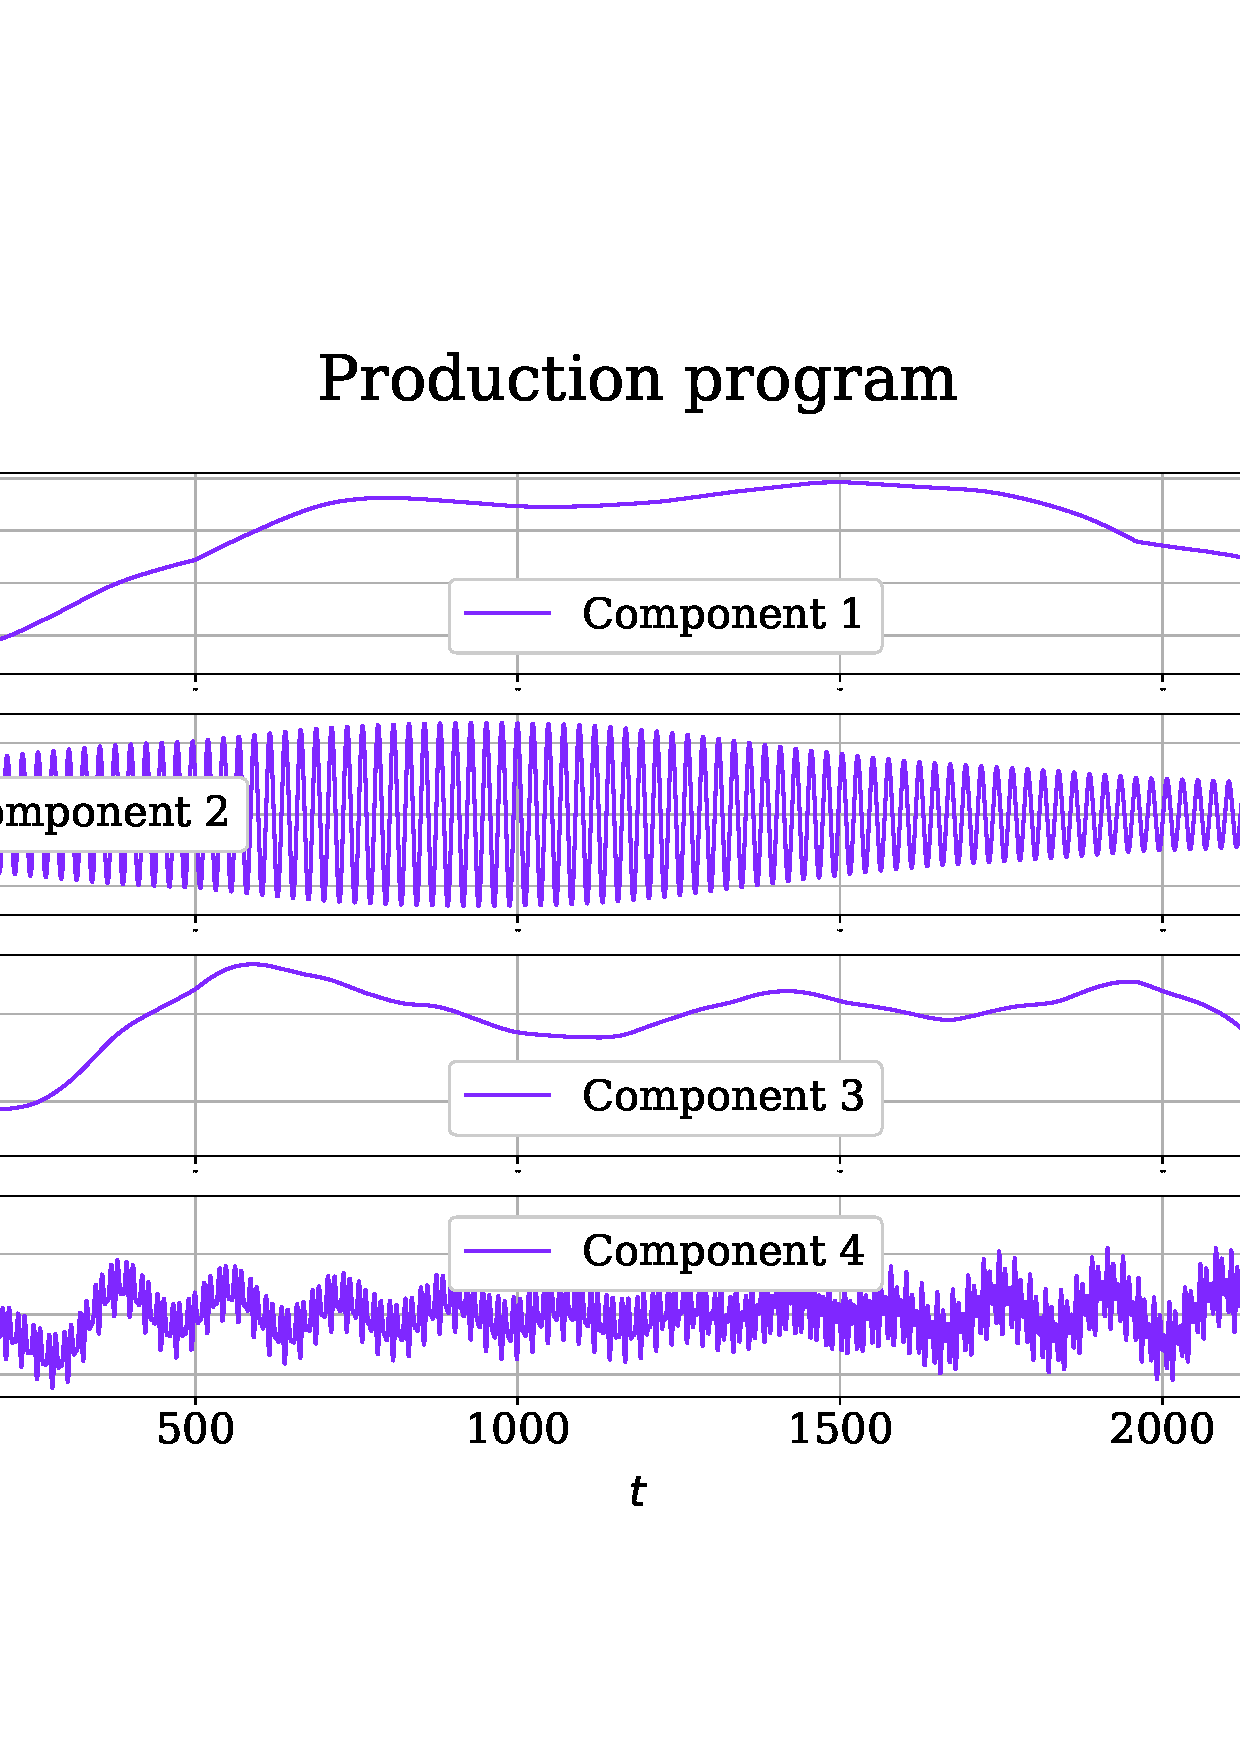
\includegraphics[width=0.48\textwidth, keepaspectratio]{../../experiments/electricity/mssa/figs/decomposition/manual/grouping_1/Production_program.png}
		\includegraphics[width=0.48\textwidth, keepaspectratio]{../../experiments/electricity/mssa/figs/decomposition/manual/grouping_1/Price.png}
		\caption{Разложение рядов на компоненты методом mSSA. Данные электроэнергии.}\label{fig:electr_decomp_mssa}
	\end{figure}
	
	\begin{figure}[h!]
		\centering
		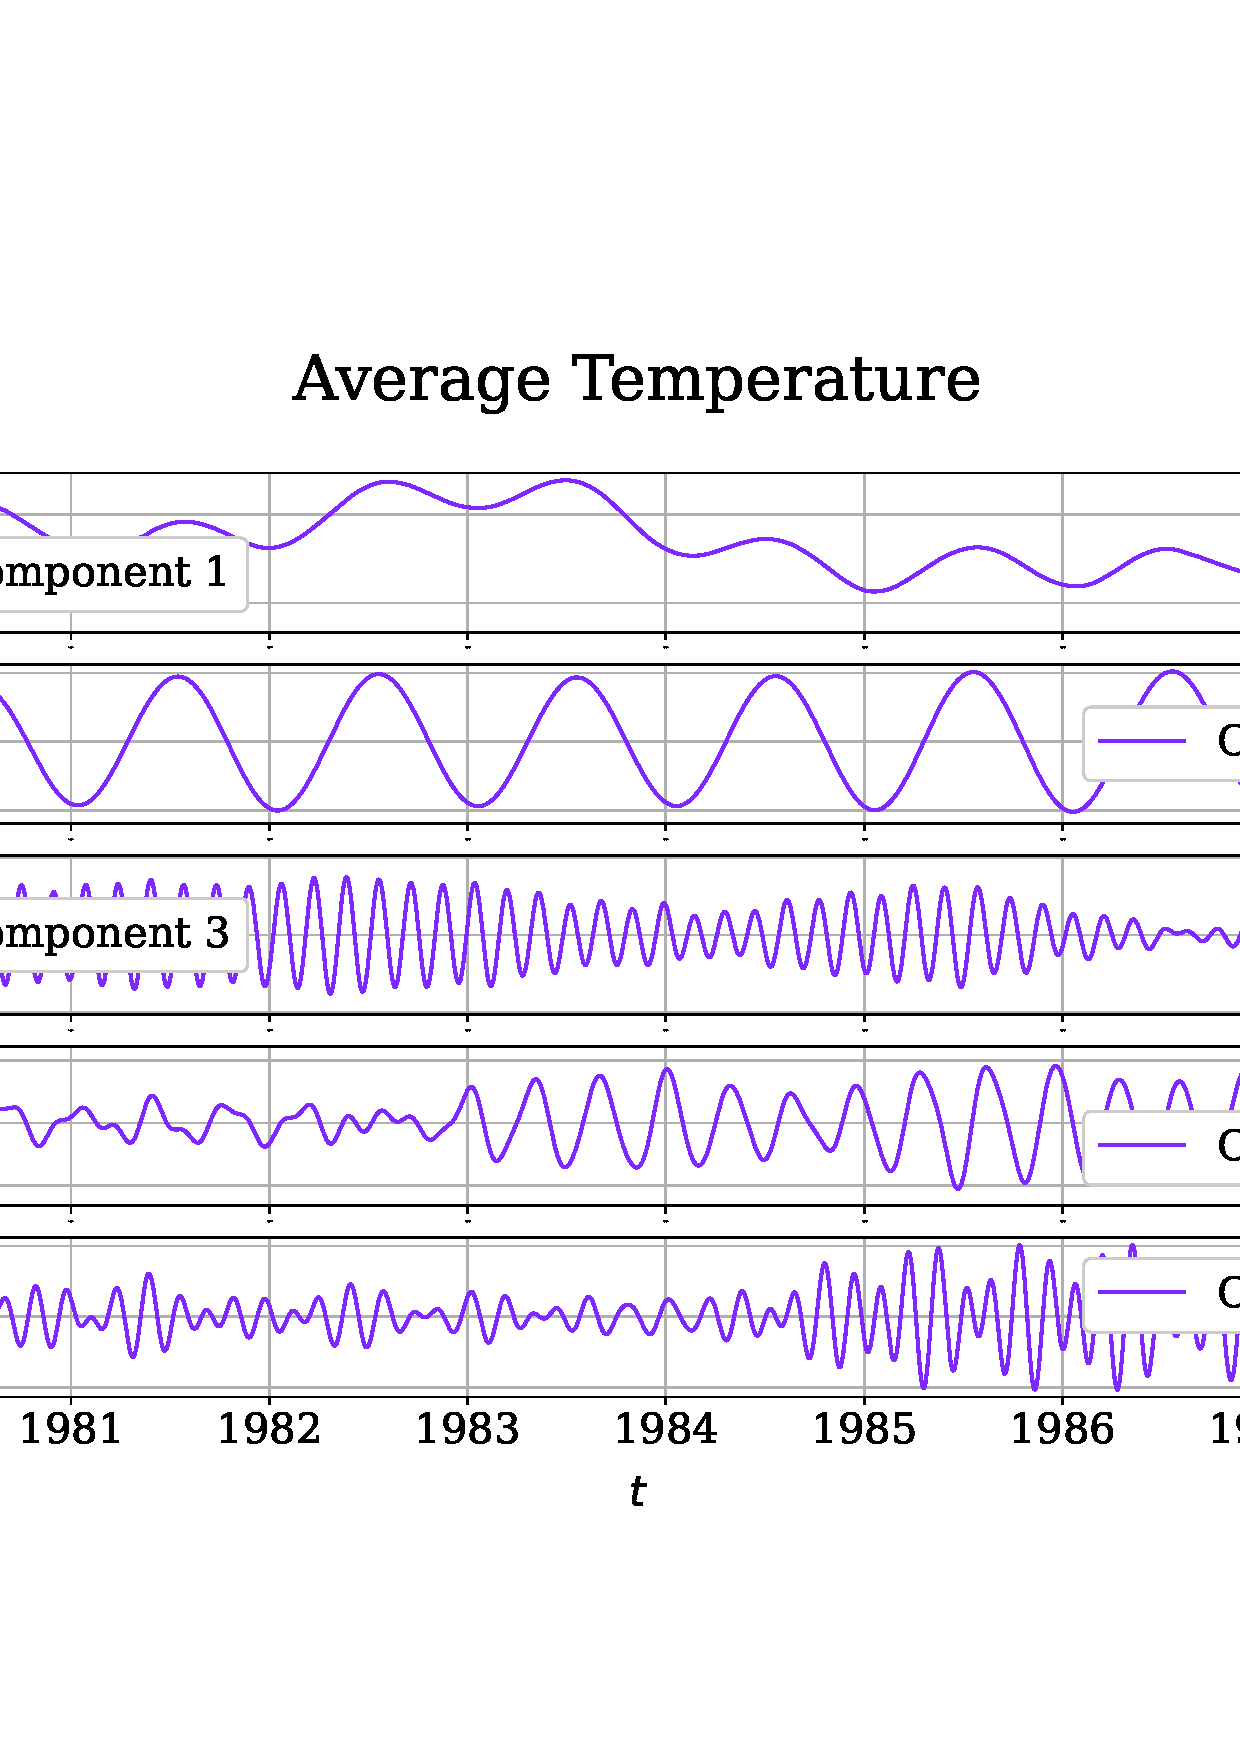
\includegraphics[width=0.48\textwidth, keepaspectratio]{../../experiments/weather/mssa/figs/decomposition/manual/grouping_1/Average_Temperature.png}
		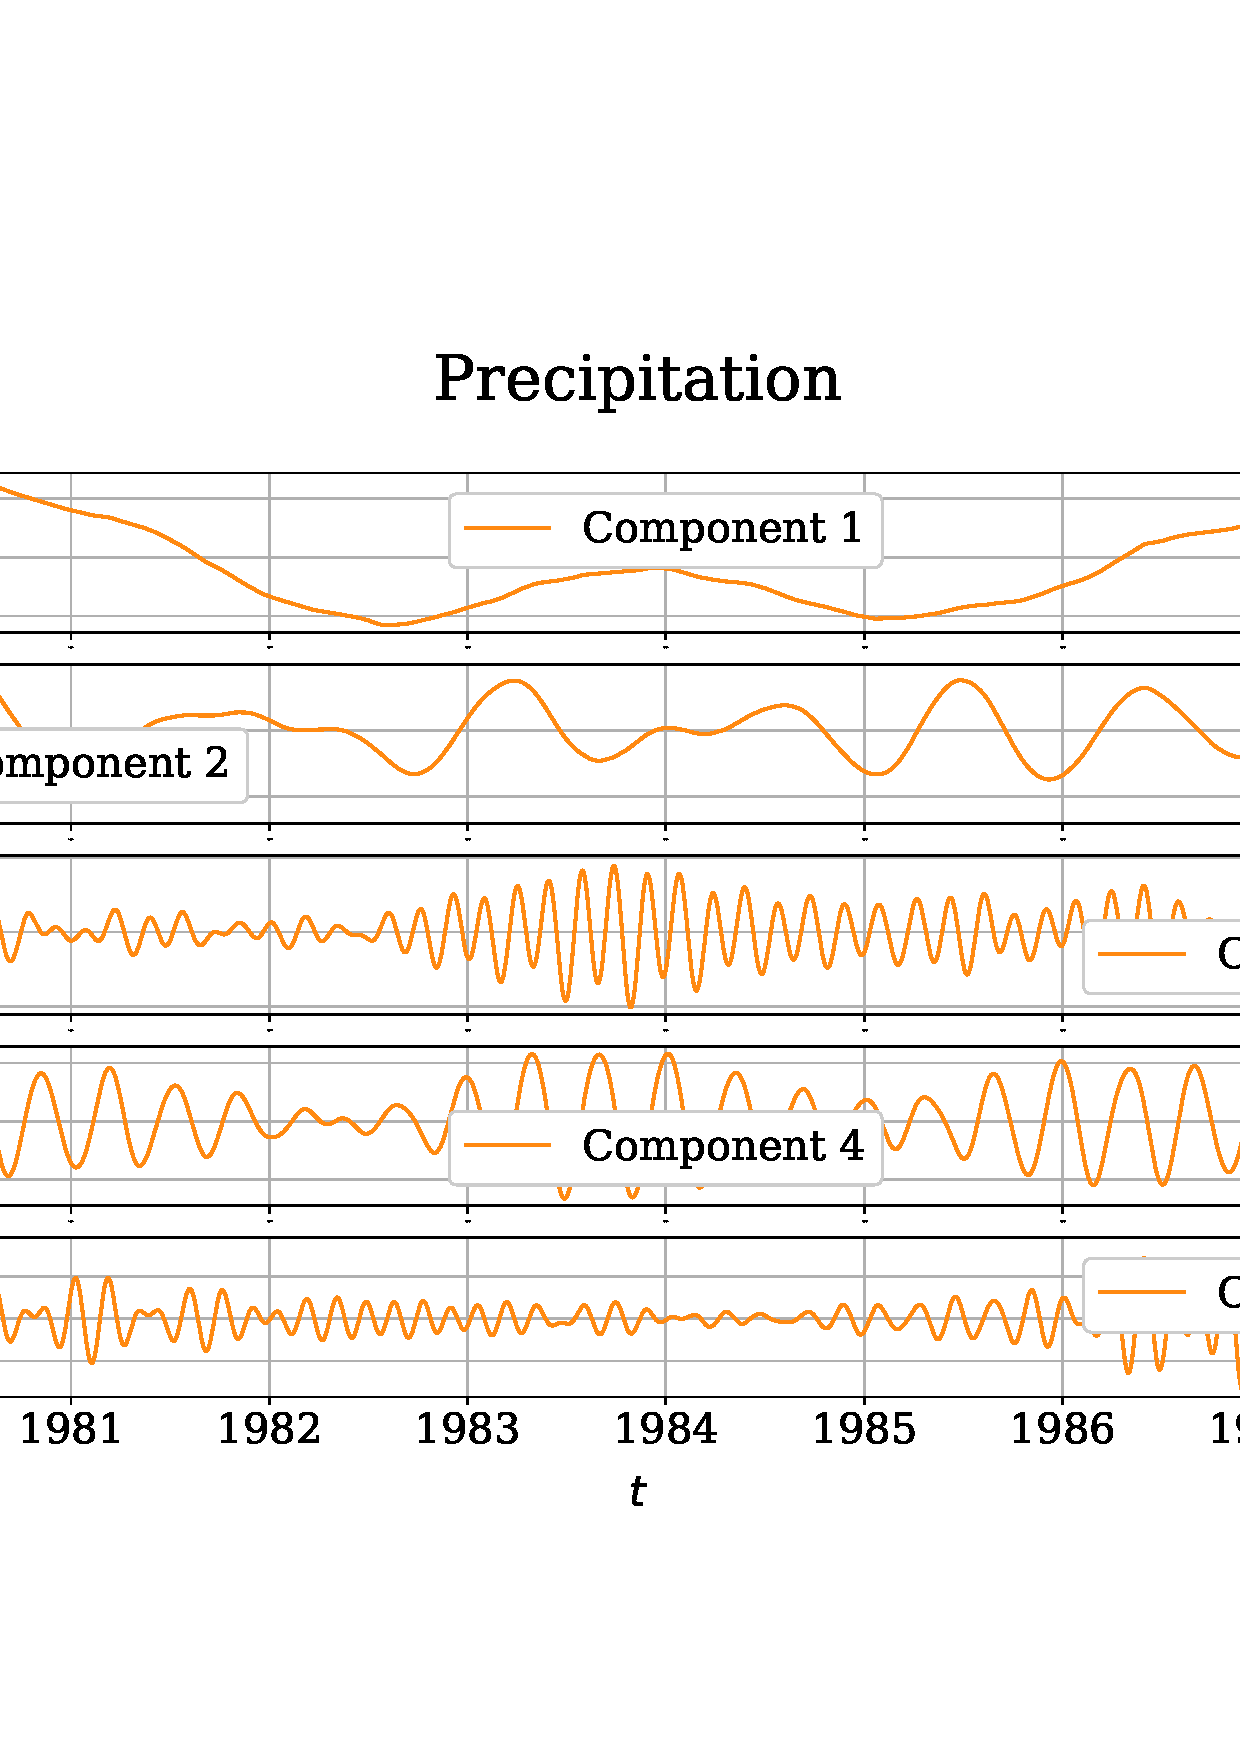
\includegraphics[width=0.48\textwidth, keepaspectratio]{../../experiments/weather/mssa/figs/decomposition/manual/grouping_1/Precipitation.png}
		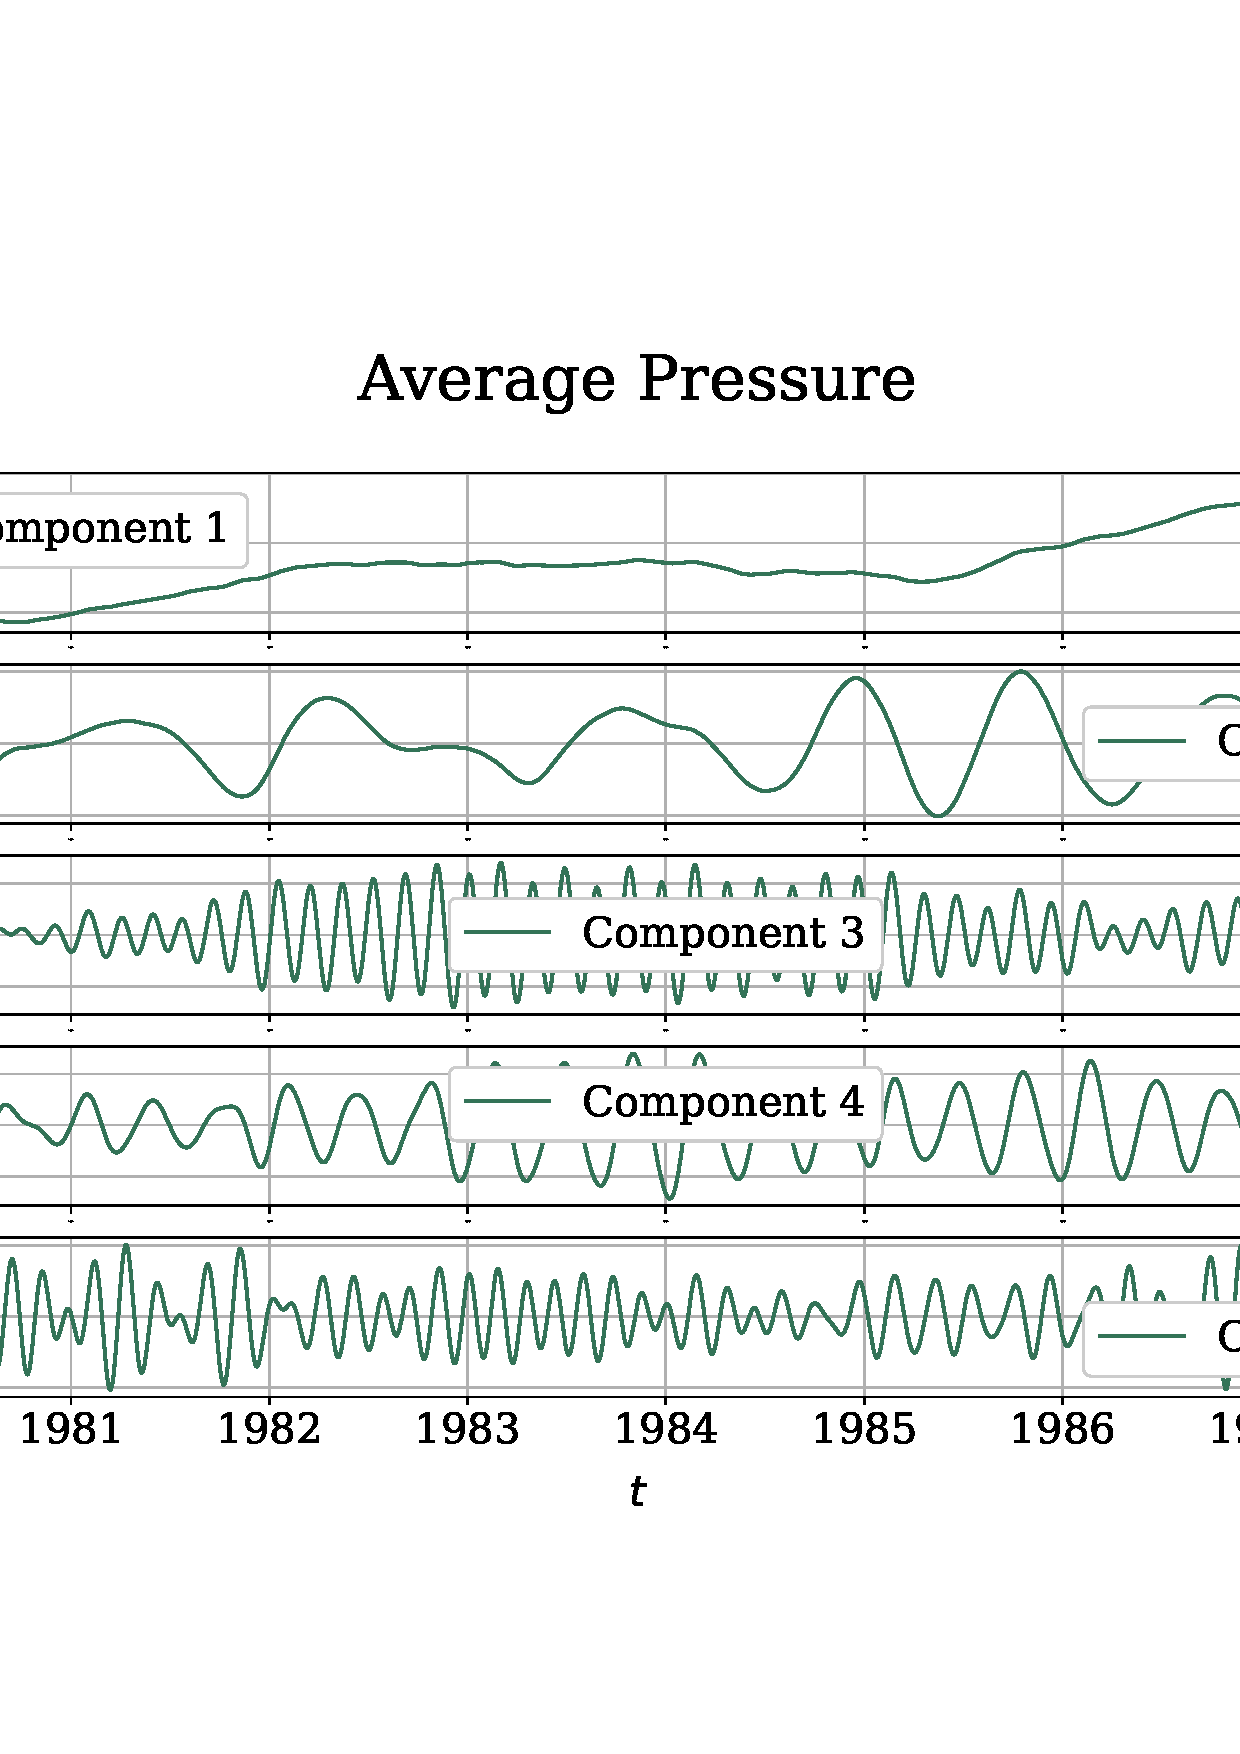
\includegraphics[width=0.48\textwidth, keepaspectratio]{../../experiments/weather/mssa/figs/decomposition/manual/grouping_1/Average_Pressure.png}
		\caption{Разложение рядов на компоненты методом mSSA. Данные погоды.}\label{fig:weather_decomp_mssa}
	\end{figure}
		
		\clearpage
		\printbibliography
	
\end{document}